\documentclass[a4paper]{report}
\usepackage[utf8]{inputenc}
\usepackage[german]{babel}
\usepackage{graphicx}

\begin{document}

\chapter{Einführung}

Die  vier Wirtschaft Subjekten:
\newline
\newline
\newline
\newline
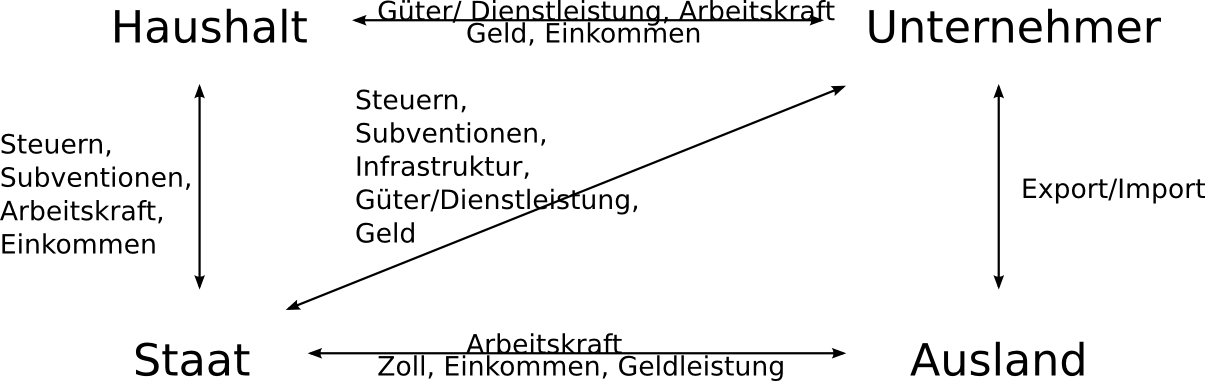
\includegraphics[scale=0.8]{image/image1.png}
\newline
\newline
\newline
\newline
Die Wirtschaftstätigkeit eines Landes wird zahlenmäßig erfasst, wobei verschiedene Ströme festgestellt werden. Zwischen den vier Wirtschaft Subjekten kommt es zu Transaktionen, Austausch von Gütern. Es gibt zwei gegenläufige Ströme:

\begin{itemize}
\item Realer Strom: Güter (Waren) und Dienstleistung
\item Monetärer Strom: Geld (Geldstrom)
\end{itemize}

Am Geldstrom wird das Volkseinkommen gemessen, am Güterstrom das Sozialprodukt. Das Sozialprodukt ist ein genereller Maßstab für die Wirtschaftskraft eines Landes. Je größer es ist, desto mehr kann im Allgemeinem verbraucht werden und desto größer ist der rechnerischer Wohlstand der Bevölkerung so fern dieser einigermaßen gleich verteilt ist.

BILD

Güter:

Einteilung der Güter nach der Verfügbarkeit:

\begin{itemize}
\item öffentliche Güter (unbegrenzt vorhanden)
\item knappe Güter (Sachgüter, Dienstleistung, Rechte, Eigentumsrecht, ...)
\end{itemize}

Einteilung der Güter nach Verwendung:

\begin{itemize}
\item Konsumgüter
	\begin{itemize}
	\item Verbrauchsgüter (für einmaligen Gebrauch z.B. Nahrung, ...)
	\item Gebrauchsgüter (für mehrmaligen Gebrauch z.B. Auto, ...)
	\end{itemize}
\item Produktionsgüter (Güter mit den sich andere Güter herstellen lassen können)
\end{itemize}

\chapter{Produktionsfaktoren}

Die vier Produktionsfaktoren sind:

\begin{itemize}
\item Boden
\item Arbeit
\item Wissen (Know-How)
\item Boden
\end{itemize}


\chapter{Taylorismus}

\chapter{Wirtschaftssektoren}


\chapter{Konjunktur Theorie}

\begin{itemize}
\item John Majuard Kaynes (1883-1946)

In den 30er Jahren kam es Aufgrund der großen Weltwirtschaftskrise zu Massenarbeitslosigkeit. Kaynes empfahl der britischen Regierung, sich bei den Banken Geld zu leihen und damit Aufträge an die Industrie zu finanzieren. Die aufgenommenen Kredite könne man dann in der folgenden Boomphase (hohe Beschäftigung $\rightarrow$ reichliche Steuereinnahmen) wieder zurückzahlen.

\item Milton Friedman (1912-2006)

In den 60er Jahren feierte der Fiskalismus glanzvolle Erfolge. Viele glaubten, man könne die Wirtschaft nach belieben ''ankurbeln'' oder ''bremsen''. In den 70er kamen zweifel auf $\rightarrow$ wirtschaftliche Stagnation, hohe Arbeitslosigkeit bzw. Inflation. Friedman war der schärfste Kritiker des Kaynsianismus. Seine Meinung nach gehört der ganze ''Sozialklingbling'' (Kinder- oder Wohngeld) abgeschafft. Er leugnet zwar nicht die Möglichkeit von Arbeitslosigkeit, weil sich nicht alle Arbeitnehmer an veränderte Strukturen anpassen können oder wollen. Außerdem muss der Staat sich das zur Ausgaben finanzierende benötigte Geld auf dem Kapitalmarkt leihen $\rightarrow$ Zinsen steigen und private Investoren werden zurückgedrängt.
\end{itemize}

\end{document}